\documentclass[12pt]{article}  
\usepackage[left=1.00in, right=1.00in, top=1.00in, bottom=1.00in]{geometry}
\usepackage{natbib}
\usepackage{setspace}
\usepackage{mathtools}
\usepackage{authblk}
\usepackage{dcolumn}
\usepackage{rotating}
\setlength{\bibsep}{0pt plus 0.3ex}
\usepackage[T1]{fontenc}
\usepackage{mathpazo}
\usepackage{graphicx}
\usepackage{booktabs}
%%\usepackage[english]{babel}
\usepackage{blindtext}
\usepackage{endnotes}
\usepackage{xr}
\externaldocument{SI}
\usepackage{multirow}
\usepackage{dcolumn}
\usepackage[usenames,dvipsnames]{xcolor}
\usepackage[colorlinks=true,
citecolor=BrickRed,linkcolor=NavyBlue]{hyperref}

\newcolumntype{d}[1]{D{.}{.}{#1}}

\externaldocument{FL_GOTV_App}

\begin{document}

\author[1]{Michael U. Rivera\thanks{We are grateful for comments from
    attendees of the 2017 State Politics and Policy Conference.}}
\author[1]{D. Alex Hughes} \author[2,3]{Micah Gell-Redman}
\affil[1]{School of Information, University of California, Berkeley}
\affil[2]{Department of International Affairs, University of Georgia}
\affil[3]{Department of Health Policy \& Management, University of
  Georgia}

\renewcommand\Authands{ and }

\title{Email Mobilization Messages Suppress Turnout Among Black and Latino Voters:\\
  Experimental Evidence From the 2016 General Election\thanks{This
    research was approved by the institutional review board of the
    University of Texas, Austin.  The data, code, and compute
    environment required to replicate all analyses in this article are
    available at the Journal of Experimental Political Science
    Dataverse within the Harvard Dataverse Network, at:
    https://doi.org/10.7910/DVN/YIZEA7 \citep{rivera2020}.}}  \date{\today}


%% anonymize IRB
\maketitle
\thispagestyle{empty}

\begin{abstract}
  \noindent \textbf{Word Count:}  1,142 \\ \\
  Email can deliver mobilization messages at considerably lower cost
  than direct mail. While voters’ email addresses are readily
  available, experimental work from 2007-2012 suggests that email
  mobilization is ineffective in most contexts. Here, we use public
  data to reexamine the effectiveness of email mobilization in the
  2016 Florida general election. Unsolicited emails sent from a
  university professor and designed to increase turnout had the
  opposite effect: emails slightly demobilizing voters. While the
  overall decrease in turnout amounted to less than 1 percent of the
  margin of victory in the presidential race in the state, the
  demobilizing effect was particularly pronounced among minority
  voters. Compared to voters from the same group who were assigned to
  control, black voters assigned to receive emails were 2.2 percentage
  points less likely to turn out, and Latino voters were 1.0
  percentage point less likely to turn out. These findings encourage
  both campaigns and researchers to think critically about the use and
  study of massive impersonal mobilization methods.

\end{abstract}

\clearpage

\setcounter{page}{1} \doublespacing

\section{Email Mobilization}

What is the effect of an unsolicited email encouragement on voter
turnout? Campaigns currently employ a broad strategy of contact that
includes both text-messages \citep{roose2018} and email
\citep{astor2019} to generate financial and electoral support. Voters
opt-in to provide their email addresses to issue-advocacy groups, and
national campaigns spend considerable effort to manage, merge, and
then re-distribute these lists for use by political allies
\citep{evers2019}. The consequence of these strategies is that voters
receive electronic communication from campaigns, though they may not
have explicitly “opted in” to receive these messages. Experiments
conducted between 2007 and 2012 are mixed in their findings about
email’s ability to generate votes (see \autoref{tab:literature}). In
this study we re-examine email mobilization because, despite little
experimental evidence in support of its effectiveness, campaigns
continue to spend considerable capital to send emails to voters for
support.

Here, we test the impact of email messages that prime social norms
about voting \citep{gerber2009}.  The messages we send emanate from a
publicly identifiable political science professor who is a member of
our research team. We contact voters using a real identity to
forestall concerns about deceptive messaging. While this experiment
was designed to test the differential impact of injunctive and
descriptive norms on turnout \citep{rivera2016}, we find no clear
evidence that voters react differently to different treatment
messages. Instead, we were very surprised to observe a small, but
persistent decrease in turnout among voters assigned to receive a
treatment message.

\begin{table}[h]
  \caption{Mixed Evidence for Email
    Mobilization \label{tab:literature}}
  \footnotesize
  \begin{tabular}{p{.3\textwidth}p{.3\textwidth}p{.3\textwidth}}
    \toprule
    \textbf{No Effect} & \textbf{Negative Effect} & \textbf{Positive Effect} \\
    \midrule
    \cite{nickerson2007} & \cite{bennion2011} & \cite{malhotra2012email} \\
    Thirteen field experiments conducted in partnership with politcal
    campaigns find emails have essentially zero effect on voter
    registration or turnout.
                       & University administrators' email
                         encouragement of students to register
                         to vote slightly decreases registration
                         rates.
                                                  & Email messages sent
                                                    from the registrar
                                                    of voters can have
                                                    small, but
                                                    significant
                                                    positive effects
                                                    on turnout.  \\ 
    \bottomrule
  \end{tabular}
  {\raggedright \footnotesize When email has been effective the senders were a trusted, offical
    source \citep{malhotra2012email}. Outside of email mobilization there is
    evidence that some efforts meant to increase turnout can
    inadvertently have the opposite effect \citep[e.g.][]{mccabe2015,
      kousser2007, grose2008, cornwall2012}.\par}
\end{table}

% Stollwerk 2006


\section{Experimental Setting, Approach, and Data}

We target voters who provide a valid email in the publicly available
October 10, 2016 Florida Division of Elections voter roll. Random
assignment to receive an email message was blocked on congressional
district and self-reported race (See Table 2 in the SI). Of the more
than 12 million registered voters in Florida, 503,859 provide a valid
email and are assigned to a condition \citep{rivera2020}.

Of all votes cast during the 2016 general election in Florida, 39.7\%
were cast early in-person, 29.4\% were by-mail, and 30.5\% were cast
in-person on election day. Throughout the reported results, the
analytic sample is the group of $328,181$ Florida voters who provide a
valid email address and did not vote early in-person. We include those
who voted by mail, because some of these voters could have sent in
their ballot after receiving a message. We exclude voters who cast a
ballot early in-person, because these votes were cast before the
distribution of our treatment messages. The analytic sample is notably
younger than the whole set of registered voters, but otherwise broadly
similar in terms of party affiliation, gender identification, and
ethnic/racial identification (\autoref{tab:email_compare}, columns 1
\& 4).


% Table created by stargazer v.5.2 by Marek Hlavac, Harvard University. E-mail: hlavac at fas.harvard.edu
% Date and time: Fri, Dec 06, 2019 - 11:27:26
\begin{table}[t]
  \begin{center}
    \caption{Comparison of Email Providers}
    \label{tab:email_compare}
    \begin{tabular}{@{\extracolsep{5pt}} rd{2}d{2}d{2}d{2}}
      \toprule
      \multirow{2}{1.25cm}{}
      & Registered & Provide & Assigned\textrm{ } A & Analytic \\
      & Voters       & Email    & Condition    & Sample   \\
      \midrule
      Proportion Democrat & $0.51$ & $0.52$ & $0.52$ & $0.51$ \\
      Age in 2016 & $51.52$ & $45.73$ & $45.50$ & $45.3$ \\ 
      Proportion Female & $0.53$ & $0.52$ & $0.52$ & $0.52$ \\
      Proportion non-White & $0.29$ & $0.31$ & $0.32$ & $0.30$ \\
      \hline \\ [-1.8ex]
      Observations & $12,339,702$ & $629,738$ & $503,859$ & $328,181$ \\
      \bottomrule
    \end{tabular}
  \end{center}
  {\linespread{1} \footnotesize \textit{Notes:} SEs are omitted here but reported in
    the SI.  \textit{Proportion Democrat} is the proportion of
    registered Democrats among those registered as a Democrat or
    Republican. %\textit{Likely Voter} is the proportion of individuals
    % who have voted in any election between 2012 and 2016.
    Column 2, \textit{Provide Email} includes registered voters with
    email addresses that could not be reconciled to be valid,
    \textit{Assigned A Condition}, includes only voters with 
    a valid email. The \textit{Analytic Sample}, used
    throughout the reported analysis, excludes voters who voted
    early in-person.} 
\end{table}


We contact voters via a single email sent from an active email address
with a .edu top-level domain. All emails contain the subject heading
``Please Remember to Vote Tomorrow'', begin with a greeting, and close
with a brief paragraph that directs questions about the voting process
to the Florida Department of State.\footnote{The SI contains
  additional details about message language, sending infrastructure,
  randomization, and data capture.}  In line with current campaign
practices, we sent messages the morning of November 7, 2016 at 10am
EST, one day before the election. Limitations on the sending
infrastructure precluded the ability to measure whether a voter
received or opened our emails \citep{hughes2019}. All results are
intent-to-treat effects.

\section{Results}

Outcome data are drawn from the June 14, 2017 official voter roll.
Voters assigned to receive no contact -- i.e. the control group --
turned out to vote at a rate of 78.7 percent (see SI Section
4.1.1).\footnote{At a target power of 0.8, this sample and design can
  detect a difference in the rates of turnout as small as 0.3
  percentage points -- roughly half the size of the established effect
  size of direct-mail (see SI Section 3.5).}  Our main experimental
finding, shown in \autoref{fig:subgroup}, is that those who were
randomly assigned to receive any email message turned out at a 0.53
percentage point lower rate ($\bar{\tau} = -0.53$, robust
$SE = 0.17$).\footnote{All estimates use robust standard
  errors and are reported as percentage points. Details of the estimation and accompanying regression
  results are provided in SI, Section 4.1.2 We find no evidence of
  differential effects across message variants (see SI Section 4.2.1
  for details). Throughout the main text, we compare the turnout of
  voters assigned to control to those assigned any message, and denote
  this treatment as $\bar{\tau}$. }

We further examine the effect of email messages within groups of
self-identified black, Latino, and white voters.\footnote{See SI
  Section 4.3 for details about estimation within subgroups.  See SI
  Table 7 for a test for heterogeneous response to treatment between
  racial/ethnic groups.}  Among the 36,518 black voters in the
analytic sample, 64.0 percent assigned to the control group voted,
compared to 61.8 percent in the treatment group
($\bar{\tau}_{b} = -2.168$, robust $SE = 0.585$). Among the 63,404
Latino voters in the analytic sample, 73.9 percent assigned to the
control group voted, compared to 73.0 percent in the treatment group
($\bar{\tau}_{l} = -0.970$, robust $SE = 0.414$).  Finally, among the
204,054 white voters in the analytic sample, 84.0 percent assigned to
the control group voted, compared to 83.7 percent in the treatment
group ($\bar{\tau}_{w} = 0.309$, robust $SE = 0.193$). Plainly stated,
these messages may have kept as many as 1,389 voters from going to the
polls ($95\%\textrm{ robust CI} = [-2249, -531]$).

\begin{figure}[t]
  \centering
  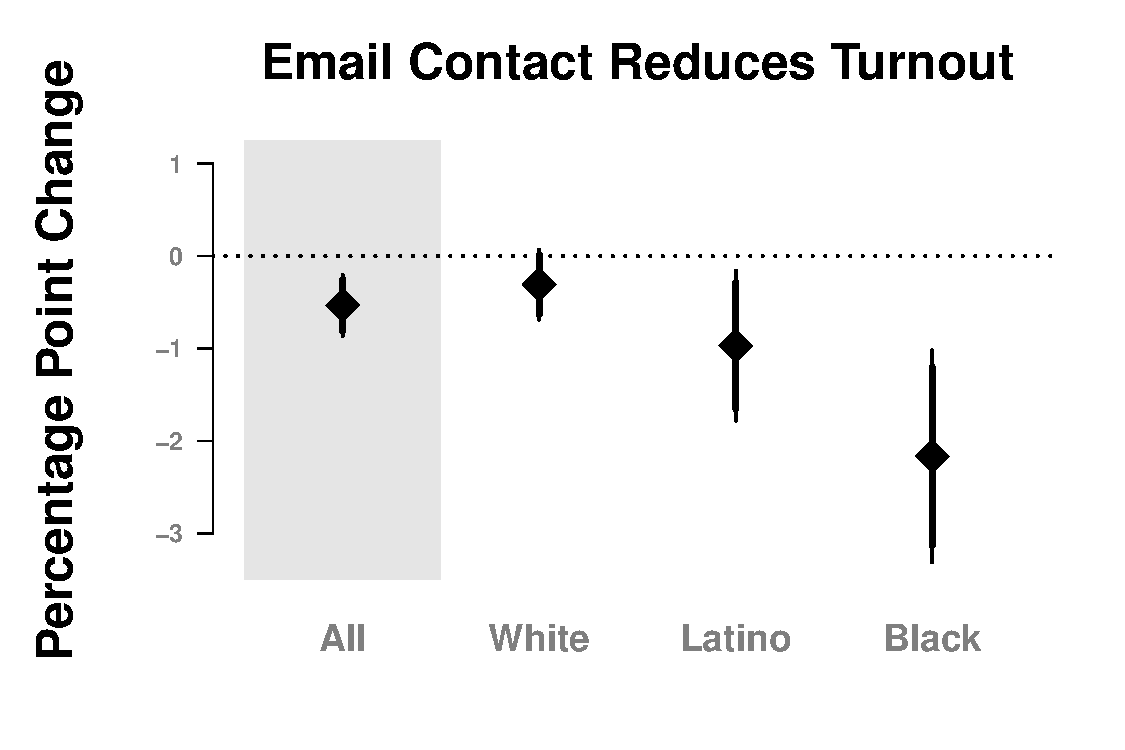
\includegraphics[width=.75\textwidth]{../tables-figures/figure_1}
  \caption[Subgroup Effect Plot]{Reduction in rate of turnout among
    registered voters assigned to receive an email, compared to voters
    of the same race/ethnicity in the control group. All points are
    estimated in separate models, on data partitions noted on the
    x-axis. Thick lines are 1.64 times the robust standard error; thin
    lines are 1.96 times the robust standard error. See Table 4 and
    Table 6 in the SI. \label{fig:subgroup}}
\end{figure}
  

\section{Discussion}

Email mobilization has attracted interest in part because of its
potential to deliver results at very low cost. Our results show that
this low-cost investment for campaigns may yield zero or even negative
returns for some groups of voters. Like all field experiments, ours
has idiosyncratic context and design features that require care in
extrapolating to both existing findings and future contexts
\citep{bates2017generalizability}. Specifically, our treatment
messages were sent in the competitive 2016 election by a university
professor with no personal or institutional connection to voters in
the study. The African American voters who received our messages live
in the shadow of twin legacies of exclusion. Not only have black
voters been shut out of the political process \citep{dawson1995}, but
the black community has also been excluded from, and in the extreme,
exploited by the research community \citep{brandt1978}. In fact, one
explanation for the particularly sharp depressive effect of our
message among these voters is a lingering mistrust of academic
researchers, especially those who lack a personal connection to the
community.

Ultimately, our design cannot support direct claims about why turnout
was reduced. However, our preferred conjecture is that receiving a
treatment message induced stress in some subjects. Approximately 700
voters chose to respond to our message; many of these people used
worried or anxious language. Voters' decisions to reply occur after
exposure to treatment, and so we are circumspect about the causal
inferences permitted by these responses \citep{coppock2019}. It is
possible, however, that when voters perceive the political environment
to be hostile or unfavorable the circumstances of voting cause stress,
and unsolicited communication may reinforce those negative impressions
and lower voters' internal motivation to turnout
\citep{hassell2017}. This perspective is consonant with careful
observational work that demonstrates that black voters who perceive a
lower chance of electing their preferred candidate are less responsive
to mobilization efforts \citep{mcgowen2010}.

There is no clear consensus within political science over the ethical
norms that should guide experimentation
\citep[e.g.,][]{desposato2015ethics}. Our own view is that the guiding
principle of experimentation should be to avoid doing harm wherever
possible, and to balance any potential harm against the knowledge to
be gained. We expected that email messages that prime social norms
might provide a low cost means to encourage turnout, and we reasoned
that for at least some voters this would occur by increasing negative
emotions \citep{gerber2009}. On the one hand, priming norms may lower
voters’ internal motivation \citep{hassell2017} by increasing shame,
stress or anxiety \citep{panagopoulos2010, marcus2000}; on the other
hand, priming norms may increase internal motivation by increasing
pride \citep{panagopoulos2010}. The net effect of these and other
forces cannot be known in advance. Because our messages decreased
turnout, we must ask whether the study’s scientific benefits
outweighed the harm done. Our answer is that the learning strongly
reinforces findings in the literature that emphasize the importance of
personal contact and connection to the community, particularly among
minority voters.


\singlespacing \bibliographystyle{apsr} \bibliography{references}
\end{document}


